%; whizzy chapter
% -initex iniptex -latex platex -format platex -bibtex jbibtex -fmt fmt
% 以上 whizzytex を使用する場合の設定。

%     Kansai Debian Meeting resources
%     Copyright (C) 2007 Takaya Yamashita
%     Thank you for Tokyo Debian Meeting resources

%     This program is free software; you can redistribute it and/or modify
%     it under the terms of the GNU General Public License as published by
%     the Free Software Foundation; either version 2 of the License, or
%     (at your option) any later version.

%     This program is distributed in the hope that it will be useful,
%     but WITHOUT ANY WARRANTY; without even the implied warranty of
%     MERCHANTABILITY or FITNESS FOR A PARTICULAR PURPOSE.  See the
%     GNU General Public License for more details.

%     You should have received a copy of the GNU General Public License
%     along with this program; if not, write to the Free Software
%     Foundation, Inc., 51 Franklin St, Fifth Floor, Boston, MA  02110-1301 USA

%  preview (shell-command (concat "evince " (replace-regexp-in-string "tex$" "pdf"(buffer-file-name)) "&"))
% 画像ファイルを処理するためにはebbを利用してboundingboxを作成。
%(shell-command "cd image200708; ebb *.png")

%%ここからヘッダ開始。

\documentclass[mingoth,a4paper]{jsarticle}
\usepackage{kansaimonthlyreport}
\usepackage[dvips]{xy}
\usepackage{ulem}

% 日付を定義する、毎月変わります。
\newcommand{\debmtgyear}{2020}
\newcommand{\debmtgdate}{22}
\newcommand{\debmtgmonth}{8}
\newcommand{\debmtgnumber}{160}

\def\fixme#1{{\color{red}{#1}}}

\begin{document}

\begin{titlepage}

% 毎月変更する部分、本文の末尾も修正することをわすれずに

 第\debmtgnumber{}回 関西 Debian 勉強会資料

\vspace{2cm}

\begin{center}
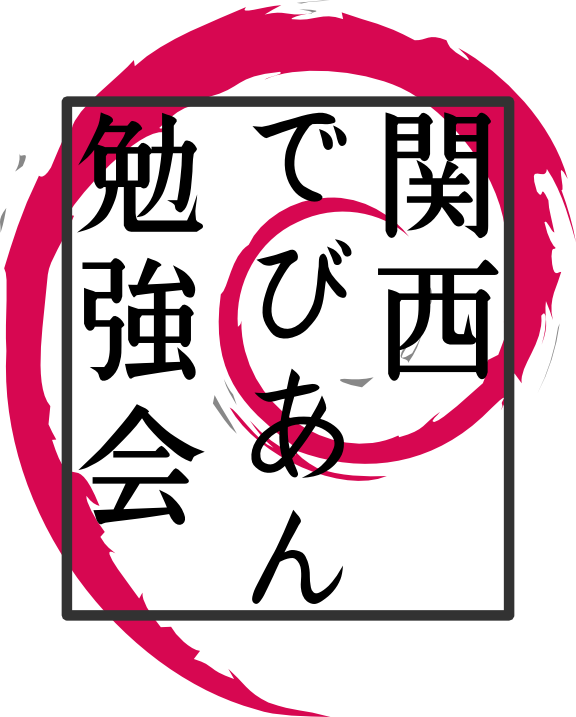
\includegraphics{image200802/kansaidebianlogo.png}
\end{center}

\begin{flushright}
\hfill{}関西 Debian 勉強会担当者 佐々木・かわだ・おおつき・小林 \\
\hfill{}\debmtgyear{}年\debmtgmonth{}月\debmtgdate{}日
\end{flushright}

\thispagestyle{empty}
\end{titlepage}

\dancersection{Makefile から CMake に高速で入門する}{Yosuke OTSUKI}

\subsection{はじめに}

CMake はkitware 社によるマルチプラットフォームで使用できるビルドツールです。
Unix 系の OS で使用されている gmake, ninja などを始め、Windows の nmake や Visual Studio の solution ファイルも出力できます。
また、unit test と .rpm や .deb 形式 \footnote{debian 公式のパッケージの規格は満たしていません。あくまでも野良パッケージです。} の作成もできます。

Go や Rust など最近のコンパイルが必要な言語は、言語独自のビルド・パッケージ機構を持っているものが多く CMake は必要ないと思います。
しかし、C/C++, Fortran など古くてコンパイルが必要な言語には便利です。
cmake は明文化されていない仕様が多く、熟練した技術者でも意外な使い方でハマることがあると思います。そこで本書では Makefile と CMakeLists.txt  を比較して cmake の習得時間を短くしようと思います。繰り返しになりますが、以下が狙いです。

\subsection{本著の狙い}
\begin{itemize}
  \item{Makefile が書ける人が、CMakeLists.txt を書けるようになる手助けをする}
  \item{CMake の明文化されてない仕様を説明して、はまらないようにする}
\end{itemize}

また、本著は CUI による cmake の使用を前提としています。IDE との連携は説明しません。\footnote{著者が cmake と IDE の連携に詳しくないのは秘密です。}
サンプルはすべて、C 言語をビルドすることにします。
ただし、パッケージングについては CMakeLists.txt のみの説明しています。
なお、本著では執筆時時点の debian buster の環境で動作確認をしています。
cmake のバージョンは 3.13.4-1 です。

note: footnote に記載しているリンクは 2020/08/21  日時の時点ではアクセスを確認しています。
\clearpage

%==============================================================================
\subsection{最初に単一ソースコードのビルド}
%==============================================================================
最初にサンプルでは C 言語のコードを単体ビルドすることにします。
そのコードをビルドする Makefile を示したあとに、同じことを CMakeLists.txt で記述した例を示します。

\vspace{1em}
C 言語のコード
\begin{commandline}
#include <stdio.h>

int main(){
    printf("Hello World\n");
    return 0;
}
\end{commandline}
\vspace{1em}
Makefile
\begin{commandline}
all: main.c
	gcc -o hello_world $?
\end{commandline}
\vspace{1em}
CMakeLists.txt
\begin{commandline}
# 必要となる最小の cmake のバージョンを指定
cmake_minimum_required(VERSION 3.13 FATAL_ERROR)

# プロジェクト名 executable の名前になる
project(hello_world)

# 文字列を標準出力に出力する。変数 CMAKE_C_COMPILER は c コンパラの絶対パス。
# cmake 実行後に生成される CMakeCache.txt の中に変数は記述される。
message ("*** ${CMAKE_C_COMPILER}")

# executable のビルド
add_executable(hello_world main.c)

# インストールのディレクトリ構成を GNU の構成にする (bin/, lib/ ...)
include(GNUInstallDirs)

# executable のみなので、bin のディレクトリをインストール対象にする
install(TARGETS hello_world DESTINATION ${CMAKE_INSTALL_BINDIR})
\end{commandline}

cmake の syntax を説明をします。
cmake\_minimum\_required は必須です。ただし、FATAL\_ERROR は省くことができます。
project で対象となる executable の名前を決めています。
add\_executable でプロジェクトのソースコードを指定し、ビルドします。
include(GNUInstallDirs) で GNU のディレクトリ構造でインストールするようにしています。
他の方法も使うことができますが、パッケージング時に絶対パスとなってしまうのでこの方法がおすすめです。

CMakeLists.txt には autools の dist clean に相当するコマンドが存在しません。
そのため、作業用のディレクトリを作りその中で cmake を呼び出します。(ここでは build という作業用のディレクトリを作ります)
そうすることで、ソースコードのディレクトリに一時的なファイルを作らなくて良くなります。
\footnote{cmake だけの用語かもしれませんが out of source build と呼ばれる方法です。}
ただし、OSS プロジェクトの中にはソースコードでビルドの実行を要求するものもあります。
以下のコマンドを実行して、autools の configure に相当することをします。

\vspace{1em}
実行コマンド
\begin{commandline}
mkdir build
cd build

# autools の configure に相当。-G で出力するビルドシステムを指定 (省略可能)
cmake -G "Unix Makefiles" -DCMAKE_INSTALL_PREFIX=`pwd`/build ../

make
make install
cd ..
\end{commandline}
正常終了すると 00.hello\_world/hello\_world が生成されます。

-G はcmake generator option です。省略するとデフォルトの Makefile が生成されます。
使用できる generator については、cmake -G で確認してください。
使用している OS によって異なります。\footnote{https://cmake.org/cmake/help/v3.18/manual/cmake-generators.7.html}

build/CMakeCache.txt を調べてみましょう。
ビルドに使用する linker, archiver や インストール先のディレクトリなどが記載されています。
中には、デフォルトで値が決まっているものもあります。
ここでは、autools の \-\-prefix に相当する CMAKE\_INSTALL\_PREFIX を使って cmake の変数の上書きについて説明します。
CMAKE\_INSTALL\_PREFIX はデフォルトでは /usr/local が値としてされています。
cmake では基本的には変数の上書きは推奨されていません。 \footnote{set(CMAKE\_INSTALL\_PREFIX /home/yosukesan PATH FORCE "") などで強制的な上書きは可能です。}
その代わりに、cmake の起動時に -D\{変数名\} として変数の初期値を与える方法が一般的です。

%==============================================================================
\subsection{外部ライブラリのリンク}
%==============================================================================

次に外部のライブラリとリンクをしてみましょう
説明のために、共有ライブラリと静的ライブラリを直接リンクします。
その後、一般的なプロジェクトで利用される共有・静的リンクどちらでも使用できる方法を紹介します。
以下の C 言語のコードのように pthread を使いたい場合を例とします。

\vspace{1em}
C 言語
\begin{commandline}
#include <pthread.h>
#include <stdio.h>

void *work(void* parg){
    int *val = (int*)parg;
    printf("worker tid=%d\n", *val);
    *val = 100;
}

int main (){
    pthread_t handle; 
    int data = 0;

    pthread_create(&handle, NULL, work, &data);    
    pthread_join(handle, NULL);
    printf("final = %d\n", data);

    return 0;
}
\end{commandline}

例えば、Makefile で共有ライブラリをリンクする場合、以下のように書きます。

\vspace{1em}
Makefile
\begin{commandline}
shared: main.c
	gcc $? -lpthread
static: main.c
	gcc $? /usr/lib/x86_64-linux-gnu/libpthread.a
\end{commandline}

\subsubsection{共有ライブラリ}

では、cmake でビルドする例を見ていきましょう。
共有ライブラリのリンクは比較的簡単に行なえます。

\vspace{1em}
CMakeLists.txt
\begin{commandline}
cmake_minimum_required(VERSION 3.13 FATAL_ERROR)

project(pthread_task)
add_executable(pthread_task main.c)

# プロジェクトとリンクするライブラリ名を指定すれば良い。システムライブラリならば、自動的に見つけてくれる。
# なお、先頭の lib は自動的に保管されるので付けてはいけない。 (libpthread.so)
target_link_libraries(pthread_task pthread)

include(GNUInstallDirs)
install(TARGETS pthread_task DESTINATION ${CMAKE_INSTALL_BINDIR})
\end{commandline}

新しく、target\_link\_library() というコマンドを使いました。
使い方については、スクリプト中のコメントを参照してください。
pthread に拡張子 (.so か .a) を付けない場合、共有ライブラリがリンクされます
cmake の実行は先の例と同じです。

\subsubsection{静的ライブラリ}

次に、静的なリンクをする方法を説明します。
共有ライブラリと異なる方法を使用します。\footnote{試した限り、共有ライブラリと同じ方法でもビルドはできました。しかし、Seg ります。これにどハマリしました。}

\vspace{1em}
CMakeLists.txt
\begin{commandline}
cmake_minimum_required(VERSION 3.13 FATAL_ERROR)

project(pthread_task)
add_executable(pthread_task main.c)

# cmake のライブラリ用のプロジェクトに外部ライブラリをインポートする。
add_library(libpthread STATIC IMPORTED)

# ライブラリの path を指定
set_target_properties(libpthread PROPERTIES IMPORTED_LOCATION /usr/lib/x86_64-linux-gnu/libpthread.a)

# ヘッダーの path を指定
set_target_properties(libpthread PROPERTIES INTERFACE_INCLUDE_DIRECTORIES /usr/include)

target_link_libraries(pthread_task libpthread)
include (GNUInstallDirs)
install(TARGETS pthread_task DESTINATION ${CMAKE_INSTALL_BINDIRS})
\end{commandline}

add\_library というコマンドを追加しました。
静的なライブラリをリンクする場合は、一度 cmake のライブラリのオブジェクトにインポートする必要が有ります。

\subsubsection{推奨する方法 find\_package()}

今までの方法では、ライブラリの絶対パスを明示的に指定してきました。
しかし、ビルドに必要な複数のライブラリの絶対パスを、全て記述するのは効率的ではありません。
また、テスト時などはインストール先を、システムパスではない PATH にするかもしれません。

そのような場合、find\_package() というコマンドを使用します。\footnote{\url{https://discourse.cmake.org/t/how-to-statically-link-external-library-by-target-link-libraries/1718}}
特定のパッケージについて、検索用の cmake スクリプトを書いておくと、find\_package() を呼び出すだけで、指定されたルートディレクトリから自動的に lib と include のパスを検索してくれます。

\vspace{1em}
CMakeLists.txt
\begin{commandline}
cmake_minimum_required(VERSION 3.13)
project(pthread_task)

# thread の中で pthread が使いたいのでフラグを立てる
set(THREADS_PREFER_PTHREAD_FLAG TRUE)

# thread ライブラリを検索。findThread.cmake が提供されているので使えるコマンド
find_package(Threads REQUIRED)

add_executable(pthread_task main.c)

# thread ライブラリをリンク
target_link_libraries(pthread_task PRIVATE Threads::Threads)

include(GNUInstallDirs)
install(TARGETS pthread_task DESTINATION ${CMAKE_INSTALL_BINDIR})
\end{commandline}

pthread のような一般的なものは、検索用のスクリプトが cmake に備わっています。\footnote{\url{https://cmake.org/cmake/help/latest/module/FindThreads.html}}
しかし、特定の用途でしか使わないライブラリの場合、例えば gmp などは自分で検索用のスクリプトを準備する必要があります。\footnote{\url{https://github.com/shohirose/cmake-find-package/blob/master/FindGMP.cmake}}
FLOSS が cmake をビルドシステムとしている場合、多くの場合検索用のスクリプトも提供される場合が多いです。
例えば、kitware 社の VTK ライブラリでは、ソースコードとともに findVTK.cmake というスクリプトが提供されています。

%==============================================================================
\subsection{分割コンパイルとリンク}
%==============================================================================

この例では、自分で作成したライブラリと自分の executable にリンクします。
この例でも共有と静的なリンクの方法を説明します。
分割コンパイルは、外部ライブラリのリンクほど難しくはありません。

整数の変数を入力引数とし、1 を加算して返す簡単な関数を自作しました。

\vspace{1em}
my\_inc.h
\begin{commandline}
#pragma once

extern int inc(int val);
\end{commandline}

\vspace{1em}
my\_inc.c
\begin{commandline}
#include <stdio.h>
#include "my_inc.h"

int inc(int val){
    printf("%d\n", ++val);
}
\end{commandline}

\vspace{1em}
main.c
\begin{commandline}
#include "my_inc.h"

int main(){
    int val = 0;
    inc(val);
    return 0;
}
\end{commandline}

\vspace{1em}
Makefile
\begin{commandline}
CFLAGS=-W -Wall
CC=gcc

.PHONY: libmyinc

all: libmyinc
	gcc $(CFLAGS) main.c libmyinc.so

libmyinc: my_inc.c
	gcc $(CFLAGS) -shared -o libmyinc.so -fPIC $?

clean:
	rm *.o *.so *.out
\end{commandline}
上記の Makefile に対応する CMakeLists.txt は以下です。
\vspace{1em}
CMakeLists.txt
\begin{commandline}
cmake_minimum_required(VERSION 3.13 FATAL_ERROR)
project(sample)

# 共有ライブラリをビルドする
add_library(my_inc SHARED my_inc.c)

add_executable(sample main.c)
target_link_libraries(sample my_inc)

include(GNUInstallDirs)
install(TARGETS my_inc DESTINATION ${CMAKE_INSTALL_LIBDIR})
install(TARGETS sample DESTINATION ${CMAKE_INSTALL_BINDIR})
install(TARGETS my_inc.h DESTINATION ${CMAKE_INSTALL_INCLUDEDIR})
\end{commandline}

動的なリンクでも、静的なリンクでもcmake の実行は先の例と同じです。
add\_library() というコマンドを追加しました。共有ライブラリを作成する場合は SHARED、STATIC と記述すると静的ライブラリが生成されます。何も記述しない場合は、共有ライブラリが生成されます。

\clearpage

%==============================================================================
\subsection{ctest で単体テスト}
%==============================================================================

自作のライブラリと自作のアプリのビルドができるようになったので、単体テストを組み込みます。
先程の、my\_inc() コマンドをテストする test() というコマンドを書いた test.c というソールコードを追加しました。このソースコードをビルドして単体テストを実行しましょう。

\vspace{1em}
test.c
\begin{commandline}
#include <stdbool.h>
#include <assert.h>

#include "my_inc.c"

bool test ()
{
    assert(inc(0) == 1);
    assert(inc(65535) == 65536);

    return true;
}

int main(){
    return test() ? 0 : -1;
}
\end{commandline}

\vspace{1em}
Makefile
\begin{commandline}
CFLAGS=-W -Wall
CC=gcc
ld_lib_path=

.PHONY: libmyinc

all: libmyinc
	gcc $(CFLAGS) main.c libmyinc.so

libmyinc: my_inc.c
	gcc $(CFLAGS) -shared -o libmyinc.so -fPIC $?

test:
	gcc $(CFLAGS) -o test.out test.c libmyinc.so
	echo -e "#!/bin/bash -x\nexport LD_LIBARY_PATH=`pwd`\n./test.out"

clean:
	rm *.o *.so *.out *.sh
\end{commandline}

\vspace{1em}
MakeLists.txt
\begin{commandline}
cmake_minimum_required(VERSION 3.13 FATAL_ERROR) 
project(sample)
add_library(my_inc my_inc.c)
add_executable(sample main.c)
target_link_libraries(sample my_inc)

enable_testing()
add_executable(test_sample test.c)
target_link_libraries(test_sample my_inc)
message ("${PROJECT_SOURCE_DIR}")
add_test(NAME unit_test COMMAND $<TARGET_FILE:test_sample> WORKING_DIRECTORY ${PROJECT_SOURCE_DIR}/build)

include(GNUInstallDirs)
install(TARGETS sample DESTINATION ${CMAKE_INSTALL_BINDIR})
install(TARGETS my_inc DESTINATION ${CMAKE_INSTALL_LIBDIR})
install(FILES my_inc.h DESTINATION ${CMAKE_INSTALL_INCLUDEDIR})

\end{commandline}

enable\_testing() と add\_test() というコマンドを追加しました。
テストを実行するために、CMAKE\_BUILD\_TYPE という変数を実行時に指定して、初期化をしています。
これは ctest を実行する場合、デフォルトの BUILD\_TYPE が実行対象に含まれないためです。 

\begin{commandline}
mkdir build
cd build
cmake -DCMAKE_INSTALL_PREFIX=`pwd`/../  -DCMAKE_BUILD_TYPE=Release ../
make

# --stop-on-failure テストに失敗したところで停止
# --verbose 詳細なメッセージを出す。実行したテストの絶対パスを表示してほしいので使っている
ctest --stop-on-failure --verbose
make install
cd ..
\end{commandline}

ctest コマンドでテストを実行します。 
引数なしでも実行は可能ですが、おすすめはサンプルの通りです。

%==============================================================================
\subsection{パッケージング}
%==============================================================================

今まで説明してきたものをすべて追加して、lib の作成、executable の作成をした後に単体テストを行い、パッケージングをするスクリプトが以下です。
CMake は正式な Debian の基準に沿った .deb は生成できません。
しかし、複数の形式のパッケージングに対応しているので社内ツールなど、それほど品質が必要ないものには便利かもしれません。

\begin{commandline}
cmake_minimum_required(VERSION 3.13 FATAL_ERROR)

project(sample)
add_library(my_inc SHARED my_inc.c)
add_executable(sample main.c)
target_link_libraries(sample my_inc)

enable_testing()
add_executable(test_sample test.c)
target_link_libraries(test_sample my_inc)
message ("${PROJECT_SOURCE_DIR}")
add_test(NAME unit_test COMMAND $<TARGET_FILE:test_sample> WORKING_DIRECTORY ${PROJECT_SOURCE_DIR}/build)

include(GNUInstallDirs)
install(TARGETS sample DESTINATION ${CMAKE_INSTALL_BINDIR})
install(TARGETS my_inc DESTINATION ${CMAKE_INSTALL_LIBDIR})
install(FILES my_inc.h DESTINATION ${CMAKE_INSTALL_INCLUDEDIR})

# prerequisite apt-get install build-essetial rpm
# .deb と .rpm をパッケージングする
set (CPACK_GENERATOR "DEB" "RPM")
set (CPACK_DEBIAN_PACKAGE_MAINTAINER "yosukesan")
set (CPACK_PACKAGE_VERSION_MAJOR "0")
set (CPACK_PACKAGE_VERSION_MINOR "1")
include (CPack)
\end{commandline}

上記の例では、.deb と .rpm を作成します。
cmake は debuild と rpmbuild を呼び出して実行するので、もしインストールしていない場合はコメント行の apt を実行してください。

上記のスクリプトを実行する場合は、以下で実行してください。
cpack でパッケージングを行っています。
今回は .deb と .rpm のみですが FreeBSD, Qt, MacOS, Windows (Wix) などにも対応しています\footnote{\url{https://cmake.org/cmake/help/v3.13/manual/cpack-generators.7.html}}。

\begin{commandline}
mkdir build
cd build
cmake -DCMAKE_INSTALL_PREFIX=`pwd`/../  -DCMAKE_BUILD_TYPE=Release ../
make
ctest
cpack
cd ..
\end{commandline}

先に説明しましたが include (GNUInstallDirs) を指定して CMAKE\_INSTALL\_\{BINDIR, LIBDIR, INCLUDEDIR\} をインストール先にしています。
このようにしないと、インストール先が絶対パスとして格納されたパッケージが出来上がってしまいます。

\subsection{まとめ}

Makefile と CMakeLists.txt を対比しつつ説明してきました。
Windows のネイティブ環境にも対応しているので、複数の OS に対してバイナリーを出力しなければならないときなどには便利です。

最後に私は以下ぐらいしか記憶していません。下記のキーワードで検索して、コマンドの仕様や、関連する仕様について cmake のドキュメントを読んだり、使用例を探したりしています。
\begin{itemize}
  \item{add\_executable() : executable のビルド}
  \item{add\_library() : ライブラリのビルド}
  \item{target\_link\_library() : executable とライブラリのリンク}
  \item{install() : make install をやるためのコマンド}
  \item{ctest, enable\_testing() and add\_test() : 単体テストに必要}
  \item{cpack : パッケージングのコマンド}
\end{itemize}

\subsection{参考文献}

\begin{itemize}
\item \url{http://opencv.jp/cmake/cmake_tutorial.html} (accessed 2020/Aug/20th)
\item \url{https://www.qoosky.io/techs/814fda555d} (accessed 2020/Aug/20th)
\item \url{https://blog.usejournal.com/creating-debian-packages-cmake-e519a0186e87?gi=1efc3589ce87} (accessed 2020/aug/20th)
\end{itemize}

\vspace{\fill}
本資料は GPL v 2.0 のライセンスで公開いたします。

\clearpage

%
% 冊子にするために、4の倍数にする必要がある。
% そのための調整

%\mbox{}\newpage
%\mbox{}\newpage

\printindex
%\cleartooddpage

 \begin{minipage}[b]{0.2\hsize}
  \rotatebox{90}{\fontsize{80}{80} {\gt 関西 Debian 勉強会} }
 \end{minipage}
 \begin{minipage}[b]{0.8\hsize}

 \vspace*{15cm}
 \rule{\hsize}{1mm}
 \vspace{2mm}
 
\includegraphics[width=2cm]{image200502/openlogo-nd.eps}
 \noindent \Large \bfseries{Debian 勉強会資料}\\ \\
 \noindent \normalfont \debmtgyear{}年\debmtgmonth{}月\debmtgdate{}日 \hspace{5mm}  初版第1刷発行\\
 \noindent \normalfont 関西 Debian 勉強会 (編集・印刷・発行)\\
 \rule{\hsize}{1mm}
 \end{minipage}

\end{document}

